\paragraph{Lema:} Dada $f:X \mapsto Y$ una función  y $\mathcal B$ una base de $Y$, entonces  $f$ es continua si y solo si $f^{-1}(B) \overset{\text{ab}}{\subseteq} X$ para todo $B \in \mathcal B$.

\paragraph{Demostración:}
\begin{enumerate}
    \item[$\Rightarrow$] O.E.M.S (Proposición de la clase 1)
    \item[$\Leftarrow$] Sea $V \overset{\text{ab}}{\subseteq} Y$, como $\mathcal{B}$ es una base de la topología de $Y$, entonces $V = \bigcup \mathcal B'$ con $\mathcal B' \subseteq \mathcal B$. Ademas:
    \begin{align*}
        f^{-1}(V) &= f^{-1}(\bigcup \mathcal B') \\
        &= \bigcup f^{-1}( \mathcal B') \\
    \end{align*}
    Con $f^{-1}(\mathcal B')$ una familia de abiertos de $X$. Por lo tanto, $f^{-1}(V)$ es abierto en $X$. Y por lo tanto, $f$ es continua.
\end{enumerate}

\paragraph{Lema}: Si $f:X \mapsto Y$  y $g:Y \mapsto Z$ son funciones continuas, entonces $g \circ f$ es continua.

\paragraph{Demostración:} Sea $V \overset{\text{ab}}{\subseteq} Z$ entonces $g^{-1}(V) \overset{\text{ab}}{\subseteq} Y$ por continuidad de $g$ y $f^{-1}(g^{-1}(V)) \overset{\text{ab}}{\subseteq} X$ por continuidad de $f$. Por lo tanto, $(g \circ f)^{-1}(V) \overset{\text{ab}}{\subseteq} X$. Por lo tanto, $g \circ f$ es continua.

\paragraph{Lema:} Si $f:X \mapsto Y$ es continua y $A$ es subespacio de $X$, entonces $f|_A$ es continua.

\paragraph{Demostración:} Sea $V \overset{\text{ab}}{\subseteq} Y$ entonces 

\begin{align*}
    f|_{A}^{-1}(V) &= f^{-1}(V) \cap A \overset{\text{ab}}{\subseteq} A
\end{align*} 
por continuidad de $f$, por la definición de la topología subespacio.

\subsection{Homoeomorfismo:}

\paragraph{Definición:} Una función $f:X \mapsto Y$ es un homeomorfismo si es biyectiva y continua y su inversa también es continua.

\paragraph{Ejemplo de NO homeomorfismo:}  La funcion $\operatorname{id}:(\mathbb R,\mathcal{T_d}) \mapsto (\mathbb R,\mathcal{T_d})$ no es un homeomorfismo, ya que la inversa no es continua.

\paragraph{Definición (Conjuntos homeomorfos):} Dados dos espacios topológicos $X$ y $Y$, decimos que son homeomorfos si existe un homeomorfismo entre ellos, y lo notamos como $X \simeq Y$.

\paragraph{Ejemplo :} En $\mathbb R^n$ con la métrica usual, para todo $\epsilon > 0$:

\begin{align*}
    B_\epsilon(x)  \simeq B_\epsilon(y) \simeq B_\epsilon(z)
\end{align*}

\subsubsection{Propiedades y ejercicios}

\begin{itemize}
    \item Demostrar que $B_\epsilon(x) \simeq B_\epsilon(y)$.  
    \begin{figure}[H]
        \centering
        \shorthandoff{>}
        %------------------------------------------------------------------
        % Dibujo TikZ
        \begin{tikzpicture}[
            scale=1.1,
            ball/.style  ={dashed, draw=red!70, very thick},
            vect/.style  ={->,   red!70, thick},
            ang/.style   ={draw=red!70, thick}
        ]
            %-----------------  Bola B_\varepsilon(x)  --------------------
            \coordinate (x) at (0,0);           % centro
            \def\r{1.5}                         % radio = \varepsilon
            \draw[ball] (x) circle (\r);        % circunferencia discontinua
    
            % Vector radial y punto sobre la frontera
            \coordinate (p) at (60:\r);         % punto a 60° sobre el círculo
            \draw[vect] (x) -- (p);
            \fill[red!70] (p) circle (0.055cm); % puntito en el extremo
    
            % Etiquetas
            \node[below left] at (x) {$x$};
            \node[red!70, above right] at (p) {$\varepsilon$};
            
            % Arco que denota el ángulo \theta
            \draw[ang] (10:0.45) arc (10:60:0.45);
            \node at (35:0.7) {$\theta$};
    
            %------------------  Flecha de "transformación" ---------------
            \draw[vect] (\r+0.8,0) -- (\r+2,0);
    
            %------------------  Sistema de ejes a la derecha -------------
            \coordinate (O) at (\r+2.8,-1);
            \draw[->] (O) -- ++(0,2) node[above] {$y$};
            \draw[->] (O) -- ++(2,0) node[right] {$x$};
    
            % Gráfica ilustrativa: recta y = x (primer cuadrante)
            \draw[->, red!70, thick] (O) -- ++(1.6,1.6);
        \end{tikzpicture}
        \shorthandon{>}
    
        %------------------------------------------------------------------
        \caption{Relación geométrica entre la bola abierta \(B_\varepsilon(x)\)
                 y su representación gráfica}
    \end{figure}
    
    \noindent\textbf{Interpretación geométrica y relación con el homeomorfismo radial:}
    
    El diagrama ilustra cómo cada punto $v$ de la bola abierta $B_{\varepsilon}(x)$ puede describirse por su dirección $\omega\in S^{n-1}$ (ángulo $\theta$ en el dibujo) y su distancia radial $r=\|v-x\|<\varepsilon$. 
    \begin{itemize}
      \item La curva en rojo marca el ángulo entre el vector radial $xv$ y el eje horizontal, representando la preservación de la dirección en el homeomorfismo.
      \item El homeomorfismo se define por 
        \[
          \Phi(v)=\frac{v-x}{\varepsilon-\|v-x\|}\in\mathbb{R}^n,
        \]
        de modo que mientras $r\to\varepsilon^{-}$, la imagen $\|\Phi(v)\|\to\infty$, rellenando todo $\mathbb{R}^n$.
      \item El sistema de ejes a la derecha simboliza $\mathbb{R}^n$, al que se envía el punto radial estirado.
      \item Este estiramiento radial es continuo y bijectivo, y su inversa
        \[
          \Phi^{-1}(w)=x+\frac{\varepsilon\,w}{1+\|w\|}
        \]
        también lo es, demostrando que $B_{\varepsilon}(x)\simeq\mathbb{R}^n$.
    \end{itemize}
    \item Demostrar que $B_\epsilon^{d_\infty}(\mathbf x) \simeq B_\epsilon^{d_1}(\mathbf x) \simeq B_\epsilon^{d_u}(\mathbf x)$.
    \item Sea $X = (a,b) \sqcup (c,d)$ con la topología usual satisface que $X \not\simeq \mathbb R$ (La prueba se hará en el futuro)
\end{itemize}

\subsubsection{Algunas superficies} 

\paragraph{N-sphera}: Sea $S^n = \{\mathbf x \in \mathbb R^{n+1} : \|\mathbf x\| = 1\} \subseteq \mathbb R^n$, la esfera de dimensión $n$ en $\mathbb R^{n+1}$. Por ejemplo:

\begin{itemize}
    \item $S^0 = \{-1,1\}$
    \begin{figure}[H]
        \centering
        % Diagrama de S^0
        \shorthandoff{>}
        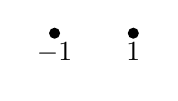
\begin{tikzpicture}[scale=1]
            \coordinate (A) at (-0.5,0);
            \coordinate (B) at (0.5,0);
            \fill (A) circle (2pt) node[below] {$-1$};
            \fill (B) circle (2pt) node[below] {$1$};
        \end{tikzpicture}
        \shorthandon{>}
    \end{figure}
    \item Circulo unitario $S^1 = \{(x,y) \in \mathbb R^2 : x^2 + y^2 = 1\}$
    \begin{figure}[H]
        \centering
        % Diagrama de S^1
        \shorthandoff{>}
        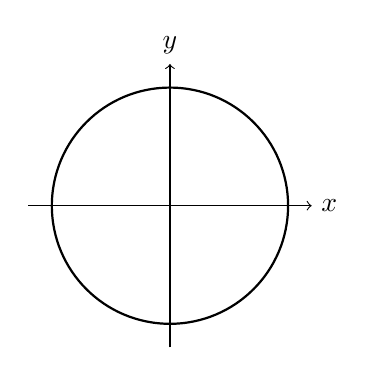
\begin{tikzpicture}[scale=1.5]
            \draw[thick] (0,0) circle (1);
            \draw[->] (-1.2,0) -- (1.2,0) node[right] {$x$};
            \draw[->] (0,-1.2) -- (0,1.2) node[above] {$y$};
        \end{tikzpicture}
        \shorthandon{>}
    \end{figure}
    \item Cascarón esférico $S^2 = \{(x,y,z) \in \mathbb R^3 : x^2 + y^2 + z^2 = 1\}$ 

    \begin{figure}[H]
        \centering
        % Diagrama de S^2
        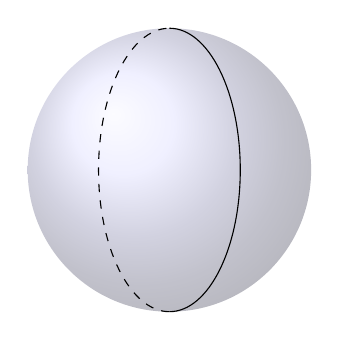
\begin{tikzpicture}[scale=1.2]
            \shade[ball color=blue!20,opacity=0.4] (0,0) circle (1.5);
            \draw (0,-1.5) arc (-90:90:0.75 and 1.5);
            \draw[dashed] (0,-1.5) arc (270:90:0.75 and 1.5);
        \end{tikzpicture}
    \end{figure}
    \item $S^n$ con la topología de subespacio de $\mathbb R^{n+1}$ es compacto, pero $\mathbb R^k$ no es compacto para todo $k \geq 1$. Es decir:

    \begin{align*}
        S^n \neq \simeq \mathbb R^k \quad \forall k \in \mathbb N \qquad (\text{la prueba se hará en el futuro})
    \end{align*}

    \item  $\mathbb R^k \simeq \mathbb R^m$ si y solo si $k=m$, esta pregunta se responde en cursos de topología algebraica. 
    \item La superficie toroidal dos dimensional $T$ representada como:  
%--- Toro animado (wireframe progresivo) ----------------------------------
\begin{figure}[H]
  \centering
      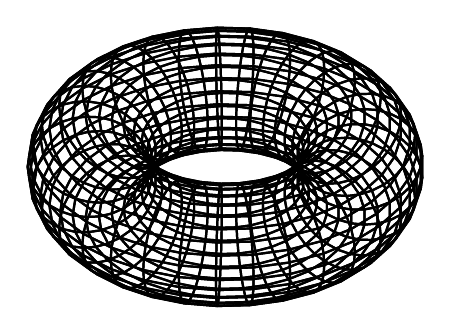
\begin{tikzpicture}
        % Parámetros del toro
        \pgfmathsetmacro{\R}{4}   % radio mayor
        \pgfmathsetmacro{\r}{1.8} % radio menor
        \begin{axis}[
          hide axis,
          view={60}{35},
          axis equal image,
          domain=0:360,
          y domain=0:360,
          samples=30,
          samples y=34,
          line join=round,
        ]
          \addplot3[
            mesh, thick, black
          ](
            {(\R + \r*cos(x)) * cos(y)},
            {(\R + \r*cos(x)) * sin(y)},
            {\r * sin(x)}
          );
        \end{axis}
      \end{tikzpicture}
    \caption{Animación de la superficie toroidal aumentando progresivamente su sección (y domain).}
\end{figure}
    satisface que:
    \begin{enumerate}[label=(\alph*)]
        \item $T\not\simeq \mathbb R^2$ \qquad \text{(la prueba se hará en el futuro)} (Ejercicio)
        \item $T \not\simeq S^2$, El toro no simplemente conexo, pero $S^2$ sí lo es.
    \end{enumerate}
    \item $\mathbb R^2 \not\simeq \mathbb R^3$
    \paragraph{Demostración:} Por contradicción, supongamos que existe un homeomorfismo $f:\mathbb R^2 \mapsto \mathbb R^3$, entonces la función $\overline f$ definida como:
    \begin{align*}
        \overline f: \mathbb R^2/\{(0,0)\} \mapsto \mathbb R^3/\{f(0,0)\} \\
    \end{align*}
    Es un homeomorfismo, que envía un conjunto que no es simplemente conexo ($\mathbb R^2/\{(0,0)\}$) a otro que sí lo es ($\mathbb R^3/\{f(0,0)\}$). 
  % ------------------------------------------------------------------
% Requiere:   \usepackage{tikz}
% (opcional)  \usetikzlibrary{arrows.meta,decorations.markings}
% ------------------------------------------------------------------
\begin{figure}[H]
    \centering
    \shorthandoff{>}
    \begin{tikzpicture}[scale=1.2,>=Stealth,
                        every node/.style={font=\scriptsize}]
      %--------------------------------------------------
      %  (1)  Plano  R^2 \ {0}  –– lazo no contractible
      %--------------------------------------------------
      % Ejes
      \draw[-] (-1.6,0) -- (-0.05,0);
      \draw[->] (.05,0) -- (1.6,0) node[right] {$x$};
      \draw[-] (0,-1.6) -- (0,-.05);
      \draw[->] (0,.05) -- (0,1.6) node[above] {$y$};
      % Origen quitado
      \draw (0,0) circle(1.5pt);
    %   \fill (0,0) circle(1.8pt);
      \node[below left=-2pt] at (0,0) {$0$};
      % Lazo que rodea al origen
      \draw[red,thin, thick] (0,0) ellipse (1 and 1.45) node[below right] {$\gamma$};
      % Flecha de orientación
      \draw[red,very thick,->] (0,1.45) ++(0:0) arc (90:40:1 and 1.45);
      % Texto explicativo
      \node[align=center,red] at (0,-2.1) {$\gamma$ no es\\deformable a un punto};
    
      % Flecha hacia el segundo dibujo
      \draw[->,thick] (2.5,0) -- (3.5,0) node[midway,above] {$f$};
    
      %--------------------------------------------------
      %  (2)  Espacio  R^3 \ {0}  –– lazo contractible
      %--------------------------------------------------
      \begin{scope}[shift={(5.5,0)}]
        % Ejes (proyección sencilla en 2D)
        
        \draw[->] (0,0.05) -- (0,2) node[above] {$z$};
        \draw[->] (0.05,0) -- (1.6,0) node[right] {$y$};
        \draw[->] (-0.03,-0.03) -- (-1,-1) node[below left] {$x$};
    
        % Lazo en el plano z = 1
        \begin{scope}[shift={(0,1.6)}]
            \draw[red!35,thin] (0,0) ellipse (.8 and 0.2) node[above right] {$\gamma_2$};
            \draw[red!35,thin,->] (0.8,0) arc (0:40:0.8 and 0.2);
        \end{scope} 
    
        % Flecha de contracción (baja por el eje z)
        % \draw[red,very thick,->] (0,1.4) -- (0,0.3);
    
        % Lazo encogido alrededor del origen
        % \draw[red,thick] (0,0) circle(0.18);
        \draw (0,0) circle(1.5pt);
    
        % (Opcional) “nube” para sugerir el espacio tridimensional
        % \draw[red!35,smooth cycle, tension=0.8 ]
        %     (1.4,1.4)
        %     .. controls (1.3, 0.2) and (1.5,-1.2) ..
        %     (0,-1.6)
        %     .. controls (-1.5,-1) and (-1.4,1.1) ..
        %     (0,1.6)
        %     .. controls (0.6,1.4) and (1.3,1.3) ..
        %     cycle;


            \draw[red!35, smooth cycle, tension=0.8] plot coordinates {
                (1,1)
                (.8,-0.5)
                % (0.8,1.6)
                % (0.2,1.0)
                (-1.0,-1.2)
                (-1,.8)
                (-0.4,1)
                (0.6,1.4)
            } node [below right] {$\gamma_3$};
      \end{scope}


    \end{tikzpicture}
    \shorthandon{>}
    \caption{En \(\mathbb{R}^{2}\setminus\{0\}\) el lazo \(\gamma\) rodea al
    origen y no puede contraerse; en \(\mathbb{R}^{3}\setminus\{0\}\) el mismo
    lazo se “eleva” por la tercera dimensión y se contrae hasta un punto.}
    \end{figure}
\end{itemize}

\paragraph {Problema del homeomorfismo} Dados dos espacios topológicos \(X\) y \(Y\). Son $X$ y $Y$ homeomorfos si?

\subsection{Topología producto}

Dados $X$ y $Y$ espacios topológicos. Queremos dotar a $X \times Y$ con una topología definida a partir de las topologías de $X$ y $Y$. Por lo que nos preguntamos:
\begin{align*}
        \Pi_1\colon X \times Y &\to X\\
        (x,y) &\mapsto x\\
        \Pi_2\colon X \times Y &\to Y\\
        (x,y) &\mapsto y
\end{align*}
Son funciones continuas?

\paragraph{Definición:} La topología producto en $X \times Y$ es la minima topología que hace continuas a las proyecciones $\Pi_1$ y $\Pi_2$.  La denotamos por $\mathcal T_{\text{prod}}$. Esta topología debe satisfacer las siguientes propiedades:  

\begin{enumerate}
    \item $\emptyset,X \times Y \in \mathcal T_{\text{prod}}$.
    \item Dado $U \in \mathcal T_X$, entonces $U \times Y \in \mathcal T_{\text{prod}}$,  con $U \times Y = \Pi_1^{-1}(U)$.
    \item Dado $V \in \mathcal T_Y$, entonces $X \times V \in \mathcal T_{\text{prod}}$,  con $X \times V = \Pi_2^{-1}(V)$.
\end{enumerate}

Notemos que, la siguiente familia de conjuntos no constituye una base para ninguna topología en $X \times Y$:
\begin{align*}
    \mathcal B = \{
        U \times Y : U \overset{\text{ab}}{\subseteq} X\} \cup \{X \times V : V \overset{\text{ab}}{\subseteq} Y\}
\end{align*}
Puesto que como se ven en el siguiente diagrama:

\begin{center}
\shorthandoff{>}
\begin{tikzpicture}[scale=2]
    % Axes
    \draw[->, red, thick] (-1,0) -- (2.5,0) node[right] {$x$};
    \draw[->, red, thick] (0,-1) -- (0,2) node[above] {$y$};

    % Dashed regions
    \draw[ForestGreen, thick, dashed] (-2,0.5) -- (4,0.5);
    \draw[ForestGreen, thick, dashed] (-2,1.5) -- (4,1.5);

    \draw[Orchid, dashed, thick]
        (1.5,-1) -- (1.5,2);
    \draw[Orchid, dashed, thick]
        (0,-1) -- (0,2);

    % Highlighted blue rectangle
    \fill[blue!20, pattern=north east lines, pattern color=blue] (0,0.5) rectangle (1.5,1.5);
    \draw[blue, thick, dashed] (0,0.5) rectangle (1.5,1.5);

    % Curly braces for U and V
    \draw[decorate, decoration={brace, amplitude=5pt}, green!70!black, thick]
    (0,0.5) -- (0,1.5) node[midway, left=6pt, green!70!black] {$V$};
    
    \draw[decorate, decoration={brace, mirror, amplitude=5pt}, Orchid, thick]
        (0,0) -- (1.5,0) node[midway, below=6pt, Orchid] {$U$};

    \definecolor{DarkBlue}{RGB}{0, 0, 150} % Dark blue
    
    % Point (x,y)
    \filldraw[DarkBlue] (0.75,1) circle (0.8pt);
    \node[DarkBlue, font=\small] at (0.75,0.85) {$(x,y)$};
\end{tikzpicture}
\shorthandon{>}
\end{center}

$B_1 = U \times Y = (a,b) \times \mathbb R \in \mathcal T_{\text{prod}}$ y $B_2 = X \times V = \mathbb R \times (c,d) \in \mathcal T_{\text{prod}}$, pero no es posible encontrar $B_3 \in \mathcal T_{\text{prod}}$ tal que $B_3 \subseteq B_1 \cap B_2 = (a,b) \times (c,d)$, ya que $B_3$ no puede ser de la forma $U \times V$ para $U \subseteq X$ y $V \subseteq Y$. Por lo tanto, $\mathcal B$ no es una base para la topología producto.

\paragraph{Definición (subbase)} Sea $\mathcal B$ una familia de abiertos de un espacio topológico $X$. Decimos que $\mathcal B$ es una subbase de la para topología de $X$  si:
\begin{align*}
    \mathcal B' = \{B_1 \cap \dots \cap B_l : B_i \in \mathcal B, l \in \mathbb N\}
\end{align*}
es una base para la topología de $X$.

\paragraph{Definición (topología producto)}  $\mathcal T_{\text{prod}}$ es la topología que tiene como subbase a la familia $\mathcal B$ de las franjas. Equivalentemente, es la topología que tiene como base:
\begin{align*}
    \mathcal B = \{U \times V : U \in \mathcal T_X, V \in \mathcal T_Y\}
\end{align*}
En general, si $X_1, \dots, X_n$ son espacios topológicos, a $X_1 \times \dots \times X_n$ lo podemos dotar de la topología producto que tiene como subbase:
\begin{align*}
    \mathcal B = \{\Pi_i^{-1}(V_i): \Pi_i: X_1 \times \dots \times X_n \to X_i, \text{ es la proyección, } V_i \overset{\text{ab}}{\subseteq} X_i\}
\end{align*}
$\mathcal B$ asi definido es lo que se conoce como franjas.

\paragraph{Ejemplo-ejercicio:}
\begin{enumerate}
    \item $S^1 \subseteq \mathbb R^2$ con la topología subespacio.
    \item $S^1 \times S^1 \subseteq \mathbb R^4$ con la topología producto igual a la topología de subespacio.
    \item $S^1\times S^1 \simeq T$.
\end{enumerate}

% %--- Toro animado (wireframe progresivo) ----------------------------------
% \begin{figure}[H]
%     \centering
%     \begin{animateinline}[controls, loop]{10}
%       \multiframe{19}{iPhi=1+10}{
%         \tikzexternaldisable
%         \begin{tikzpicture}
%           % Parámetros del toro
%           \pgfmathsetmacro{\R}{4}   % radio mayor
%           \pgfmathsetmacro{\r}{1.8} % radio menor
%           \begin{axis}[
%             hide axis,
%             view={60}{35},
%             axis equal image,
%             samples=30,
%             samples y=34,
%             line join=round,
%           ]
%             % Sección desde círculo interior hacia afuera
%             \addplot3[
%               mesh,
%               draw=blue,
%               thick,
%               domain=0:\iPhi,
%               y domain=0:360
%             ](
%               {(\R + \r*cos(x-180)) * cos(y)},
%               {(\R + \r*cos(x-180)) * sin(y)},
%               {\r * sin(x)}
%             );
%             \addplot3[
%               mesh,
%               draw=blue,
%               thick,
%               domain=180:180+\iPhi,
%               y domain=0:360
%             ](
%               {(\R + \r*cos(x)) * cos(y)},
%               {(\R + \r*cos(x)) * sin(y)},
%               {\r * sin(x)}
%             );
%             % Sección desde círculo interior (opuesto) hacia afuera
%             \addplot3[
%               mesh,
%               draw=red,
%               thick,
%               domain=0:360,
%               y domain=0:2*\iPhi
%             ](
%               {(\R + \r*cos(x)) * cos(y)},
%               {(\R + \r*cos(x)) * sin(y)},
%               {\r * sin(x)}
%             );
%              \addplot3[
%               domain=0:360,
%               samples=50,
%               dashed,
%               thick,
%               color=black,
%             ]
%             (
%               {(\R+\r)*cos(x)},
%               {(\R+\r)*sin(x)},
%               {0}
%             );
%           \end{axis}
%           \tikzexternalenable
%         \end{tikzpicture}
%       }
%     \end{animateinline}
%   \end{figure}


  